\documentclass[a4paper,14pt,oneside]{book}
\usepackage{fontspec}
\setmainfont{Times New Roman}


\usepackage[utf8]{inputenc}
\usepackage[T2A]{fontenc}
\usepackage[english,russian]{babel}   %% загружает пакет многоязыковой вёрстки
 
\usepackage{fontspec}      %% подготавливает загрузку шрифтов Open Type, True Type и др.
\defaultfontfeatures{Ligatures={TeX},Renderer=Basic}  %% свойства шрифтов по умолчанию
\setmainfont[Ligatures={TeX,Historic}]{Times New Roman} %% задаёт основной шрифт документа
\setsansfont{Comic Sans MS}                    %% задаёт шрифт без засечек
\setmonofont{Courier New}

\usepackage{indentfirst}
\frenchspacing   % интервалы между словами и предложениями - одинаковые

\clubpenalty=9999        %  без висячих строк
\widowpenalty=9999    %  без висячих строк

%%% Работа с русским языком
\usepackage{cmap}                   % поиск в PDF
\usepackage{mathtext}               % русские буквы в фомулах

%%% Дополнительная работа с математикой
\usepackage{amsmath,amsfonts,amssymb,amsthm,mathtools} % AMS
\usepackage{icomma} % "Умная" запятая: $0,2$ --- число, $0, 2$ --- перечисление

%% Свои команды
\DeclareMathOperator{\sgn}{\mathop{sgn}}

%% Перенос знаков в формулах (по Львовскому)
\newcommand*{\hm}[1]{#1\nobreak\discretionary{}
{\hbox{$\mathsurround=0pt #1$}}{}}

%%% Работа с картинками
\usepackage{graphicx}  % Для вставки рисунков
%\graphicspath{{images/}{images2/}}  % папки с картинками
\setlength\fboxsep{3pt} % Отступ рамки \fbox{} от рисунка
\setlength\fboxrule{1pt} % Толщина линий рамки \fbox{}
\usepackage{wrapfig} % Обтекание рисунков текстом

%%% Работа с таблицами
\usepackage{array,tabularx,tabulary,booktabs} % Дополнительная работа с таблицами
\usepackage{longtable}  % Длинные таблицы
\usepackage{multirow} % Слияние строк в таблице

%%% Теоремы
\theoremstyle{plain} % Это стиль по умолчанию, его можно не переопределять.
\newtheorem{theorem}{Теорема}[section]
\newtheorem{proposition}[theorem]{Утверждение}
 
\theoremstyle{definition} % "Определение"
\newtheorem{corollary}{Следствие}[theorem]
\newtheorem{problem}{Задача}[section]
 
\theoremstyle{remark} % "Примечание"
\newtheorem*{nonum}{Решение}

%%% Программирование
%\usepackage{etoolbox} % логические операторы

%%% Страница
\usepackage{extsizes} % Возможность сделать 14-й шрифт
\usepackage{geometry} % Простой способ задавать поля
    \geometry{top=25mm}
    \geometry{bottom=35mm}
    \geometry{left=35mm}
    \geometry{right=20mm}
 %
\usepackage{fancyhdr} % Колонтитулы
    \pagestyle{fancy}
    \renewcommand{\headrulewidth}{0mm}  % Толщина линейки, отчеркивающей верхний колонтитул
%    \lfoot{Нижний левый}
%    \rfoot{Нижний правый}
%    \rhead{Верхний правый}
%    \chead{Верхний в центре}
%    \lhead{Верхний левый}
    % \cfoot{Нижний в центре} % По умолчанию здесь номер страницы

\usepackage{setspace} % Интерлиньяж
\onehalfspacing % Интерлиньяж 1.5
%\doublespacing % Интерлиньяж 2
%\singlespacing % Интерлиньяж 1

\usepackage{lastpage} % Узнать, сколько всего страниц в документе.

\usepackage{soul} % Модификаторы начертания, highlight text

\usepackage{hyperref}
\usepackage[usenames,dvipsnames,svgnames,table,rgb]{xcolor}
\hypersetup{                % Гиперссылки
    unicode=true,           % русские буквы в раздела PDF
    pdftitle={Заголовок},   % Заголовок
    pdfauthor={Автор},      % Автор
    pdfsubject={Тема},      % Тема
    pdfcreator={Создатель}, % Создатель
    pdfproducer={Производитель}, % Производитель
    pdfkeywords={keyword1} {key2} {key3}, % Ключевые слова
    colorlinks=true,        % false: ссылки в рамках; true: цветные ссылки
%    linkcolor=[rgb]{0.047,0.023,0.121},          % внутренние ссылки  , оглавление здесь 
%    linkcolor=[rgb]{0.2,0.1,0.5},          % внутренние ссылки  , оглавление здесь
     linkcolor=[rgb]{0,0,1},          % внутренние ссылки  , оглавление здесь
%    linkcolor=[rgb]{0.1016,0.074,0.1836},          % внутренние ссылки  , оглавление здесь
%    citecolor=green,        % на библиографию
    citecolor=[rgb]{0,0,1},        % на библиографию
%    filecolor=magenta,      % на файлы
    filecolor=[rgb]{0,0,1},      % на файлы
    urlcolor=[rgb]{0,0,1}           % на URL
%    urlcolor=cyan           % на URL
}

%\renewcommand{\familydefault}{\sfdefault} % Начертание шрифта

\usepackage{multicol} % Несколько колонок

%\author{\LaTeX{} в Вышке}
%\title{3.2 Оформление документа в целом}
%\date{\today}
\usepackage[justification=justified,singlelinecheck=false]{caption}  % параметры - выравнивание влево
\usepackage{titlesec}    % formatting chapter title
\titleformat{\chapter}[hang] 
{\normalfont\huge\bfseries}{\chaptertitlename\ \thechapter}{1em}{}   %  word chapter and chapter name in one line

% сплошная нумерация таблиц и рисунков
\usepackage{chngcntr}   
\counterwithout{figure}{chapter}
\counterwithout{table}{chapter}

\usepackage{geometry}
\geometry{verbose,tmargin=20mm,bmargin=20mm,lmargin=30mm,rmargin=15mm}  %  margins

% списки без вертикальных интервалов по Столярову
\newenvironment{compactlist}{
\begin{list}{{$\bullet$}}{
\setlength\partopsep{0pt}
\setlength\parskip{0pt}
\setlength\parsep{0pt}
\setlength\topsep{0pt}
\setlength\itemsep{0pt}
}
}{
\end{list}
}





\usepackage{graphicx}
\usepackage{pdfpages}
\graphicspath{{pictures/}}
\DeclareGraphicsExtensions{.pdf,.png,.jpg,.bmp}


\title{обучение  LaTEX}
\author{Дмитрий Вилинский}
\date{June 2019}

\begin{document}

\begin{titlepage}
{\small
\centerline{Министерство образования и науки Российской Федерации}
\centerline{Федеральное государственное автономное образовательное учреждение}
\centerline{высшего образования}
\centerline{<<Уральский федеральный университет имени первого президента России Б.Н.Ельцина>>}
\vskip1cm
\centerline{Институт естественных наук и математики}
\centerline{Кафедра Механики и математического моделирования}
}
\vskip1cm

\null\hfill
\begin{minipage}{0.6\textwidth}
ДОПУСТИТЬ К ЗАЩИТЕ В ГЭК\\
Зав.~кафедрой\hfill \rule[-1pt]{4.5cm}{0.4pt}
$\underset{\text{(подпись)}}{\underline{\hspace{3cm}}}$
\hfill
%\hspace{4pt}
$\underset{\text{(Ф.И.О.}}{\underline{\hspace{4.5cm}}}$\\
%\hfill$\ll$\rule[-1pt]{0.5cm}{0.4pt}$\gg$\rule[-1pt]{4cm}{0.4pt} 2017г.    % кавычки елочкой командой
\hfill <<\rule[-1pt]{0.5cm}{0.4pt}>>\rule[-1pt]{4cm}{0.4pt} 2017г.
\end{minipage}\\
\vskip1cm
\centerline{\textbf{МАГИСТЕРСКАЯ ДИССЕРТАЦИЯ}}
\centerline{Изучение LaTeX}
\centerline{В сверхбыстрых темпах}
\centerline{с примерами}
\vskip3.5cm
\noindent
Научный руководитель: д.т.н., профессор Научрук\hfill $\underset{\text{(подпись)}}{\underline{\hspace{3cm}}}$\\
Консультант: Консултант1 \hfill $\underset{\text{(подпись)}}{\underline{\hspace{3cm}}}$\\
Консультант: Консультант2 \hfill $\underset{\text{(подпись)}}{\underline{\hspace{3cm}}}$\\
Нормоконтролер: Нормоконтроллер \hfill $\underset{\text{(подпись)}}{\underline{\hspace{3cm}}}$\\
Студент группы \rule[-1pt]{1.5cm}{0.4pt}  Д.А. Вилинский  \hfill $\underset{\text{(подпись)}}{\underline{\hspace{3cm}}}$\\
\vfill
\centerline{Екатеринбург}
\centerline{2019}
\end{titlepage}

\setcounter{secnumdepth}{4}
\setcounter{tocdepth}{4}
\setcounter{page}{1}
\renewcommand{\bibname}{Библиография}

\chapter*{РЕФЕРАТ}
%\addcontentsline{toc}{chapter}{РЕФЕРАТ}

\thispagestyle{empty}   % отменить вывод номера страницы
Работа будет представлять из себя описание обучения LATEX. Каждая глава это краткое или сверхраткое описание теоретической части задания на неделю, которая в тоже время является примером его выполнения (если конечно таким примером не является вся работа)
Поехали

\tableofcontents
\thispagestyle{empty} 

\chapter {Практика 1}
\setcounter{page}{4}  % номер первой страницы после оглавления
\subsection{Задание}
2019-02- Практика 1 
Задание на неделю 
\begin{enumerate}
\item Зарегистрироваться на https://www.overleaf.com: набрать тестовую статью на русском языке, пригласить меня по адресу potatocoach@gmail.com 
\item Зарегистрироваться на https://github.com: попытаться синхронизировать проект своей статьи (из предыдущего пункта) с проектом на github, пригласить меня к сотрудничеству: justjune 
\item Скачать и установить https://miktex.org 
\item Попытаться синхронизировать свою статью из п. 2 с локальным каталогом при помощи git. Исключить из синхронизации все лишние файлы каталога (при помощи настроек git). 
\item Отчитаться в OneNote на своей персональной странице: что получилось, что - нет 
\end{enumerate}
\section{Выполнение}
Итак по пунктам 
\begin{enumerate}
\item Сделанно имя учетной: an-tack@yandex.ru (соавторы как я понял не очень нужны с учетом гита)
\item Сделанно имя учетной VilinskyDA. Проект синхронизирован через локальный репозиторий]
\item Сделанно
\item см пункт 2
\item неимеет смысла в связи с несвоевременным исполнением задания
\end{enumerate}
\chapter{Практика 2}
\subsection{Задание}
2019-03-01 Практика 2 
Задание на неделю 
\begin{enumerate}
\item Ликвидировать долги первой недели 
\item Продемонстрировать в "статье" первой недели ввод сложных многострочных формул с нумерацией и без, а также вставку рисунка 
\item Продемонстрировать ссылки на все объекты в тексте 
\end{enumerate}
\section{Выполнение}
Первый пункт выполнен
\subsection{Формулы}
Приведем краткую справку о формулах \\
Общие положения.
Математические части текста внутри одного абзаца заключают или между $\backslash$( и
$\backslash$), или между \$ и \$, или между  $\backslash$begin{math} и $\backslash$end{math}. Математическими текстами считаются как полные математические формулы, так и отдельные
обозначения величин, которые относятся к формулам, греческие буквы, верхние
и нижние индексы в тексте и различные особые обозначения.\cite{LaTEX1}\\
Далее приведем примеры Бесмысленных и беспощадных Формул Из \cite{LATEX2}
\[
\lim_{n \to \infty}
\sum_{k=1}^n \frac{1}{k^2}
= \frac{\pi^2}{6}
\]
В то же время внутри абзаца $ \lim_{n \to \infty}
\sum_{k=1}^n \frac{1}{k^2}
= \frac{\pi^2}{6} $,

\[
\lefteqn{\underbrace{
\phantom{a_1+\dots+a_i+a_j}}}
a_1+\dots+\overbrace{a_i+a_j+\dots+a_n}
\]

\begin{equation} \label{eps1}
\epsilon > 0
\end{equation}
Сыылка на формулу (\ref{eps1})

Примеры использования  amsmath

\[ 
\genfrac{[}{]}{1pt}{0}{1+x}{1-x} =
\genfrac{(}{)}{}{1}{1+x}{1-x} =
\genfrac{<}{>}{}{2}{1+x}{1-x} =
\genfrac{}{}{}{3}{1+x}{1-x}
\]

Далее формулы будут номероваться с привязкой к главе 

\numberwithin{equation}{section}

\begin{equation} \label{2}
C_n^k=\binom n k=\dbinom n k=\tbinom {n k} {h-1}
\end{equation}

Матрицы

\[ \bordermatrix{
& & & j & \cr
& b_{11} & \dots & 0 & b_{1n} \cr
& \dots & \dots & 0 & \dots \cr
i & 0 & 0 & 1 & 0 \cr
& \dots & \dots & 0 & \dots \cr
& b_{m1} & \dots & 0 & b_{mn} \cr}
\]


Еще немного нумерации формул и выравнивания
\begin{align}
 x &= A^{-1}b; \tag{*Очень важная формула}\label{aster} \\
 x &> 0; \label{restr} \\
 2-x &> x_0; \tag{\ref{restr}$’$}
\end{align}
Нет ничего важнее, чем важность ~\eqref{aster}.\\
А теперь формулы с доп буквами
\begin{subequations}
\begin{equation} A=0
\end{equation}
ниже еще 2 фориулы 
\begin{gather} B=0 \\ C=0
\end{gather}
\end{subequations}

\begin{equation}
x=A^{-1}b
\end{equation}
Формула в несколько строк 
\begin{multline*}
S_n = a_1+\dots+a_n = \\
= (a_1+a_n) + (a_2+a_{n-1}) +  \dots = \\
= (a_1+a_n)\,n/2
\end{multline*}
\subsection{Изображения}
Иструкция
Для вставки рисунков понадобится пакет graphicx. Его, как и другие пакеты LaTeX, необходимо указать в преамбуле документа:\\
$\backslash$usepackage[argument]\{graphicx\}
Значение аргумента argument может быть следующим:
\begin{itemize}
\item dvips (аргумент по умолчанию при компиляции с помощью latex), если вы собираетесь компилировать документ при помощи latex для получения DVI-файла.
\item dvipdfm, если документ компилируется latex, и полученный в результате DVI-файл предполагается конвертировать в PDF при помощи dvipdfm.
\item pdftex (аргумент по умолчанию при компиляции с помощью pdflatex), если документ предполагается компилировать pdftex, чтобы непосредственно получить PDF-файл.
\end{itemize}
Теперь укажем путь к графическим файлам. Пусть они помещаются в подкаталог pictures текущего каталога \\
$\backslash$graphicspath\{\{pictures/\}\}\\
(текущим считается тот каталог, где находится наш файл *.tex).\\
Кроме того, в преамбуле можно указать список расширений, которые будут трактоваться как графические\\
$\backslash$DeclareGraphicsExtensions\{.pdf,.png,.jpg\}\\
Теперь, вставляя в документ файл одного из указанных выше типов, его расширение указывать не обязательно.\\
Вставка графических объектов\\
В текст документа графический файл вставляется командой $\backslash$includegraphics:\\
Вставим первый попавшийся график\\
\begin{figure}[h]
\center{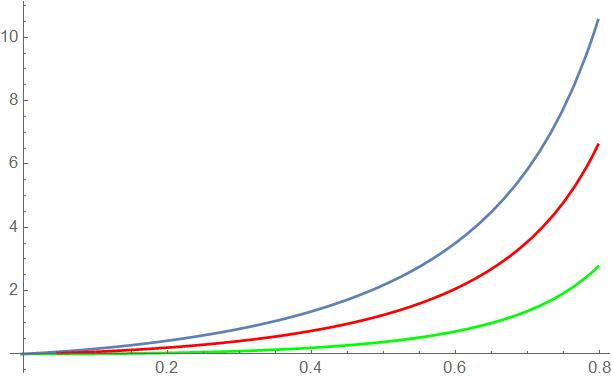
\includegraphics[width=\textwidth]{1}}
\caption{первый попавшийся график}
\label{fig:1}
\end{figure}
Вставим второй  график
\begin{figure}
\center{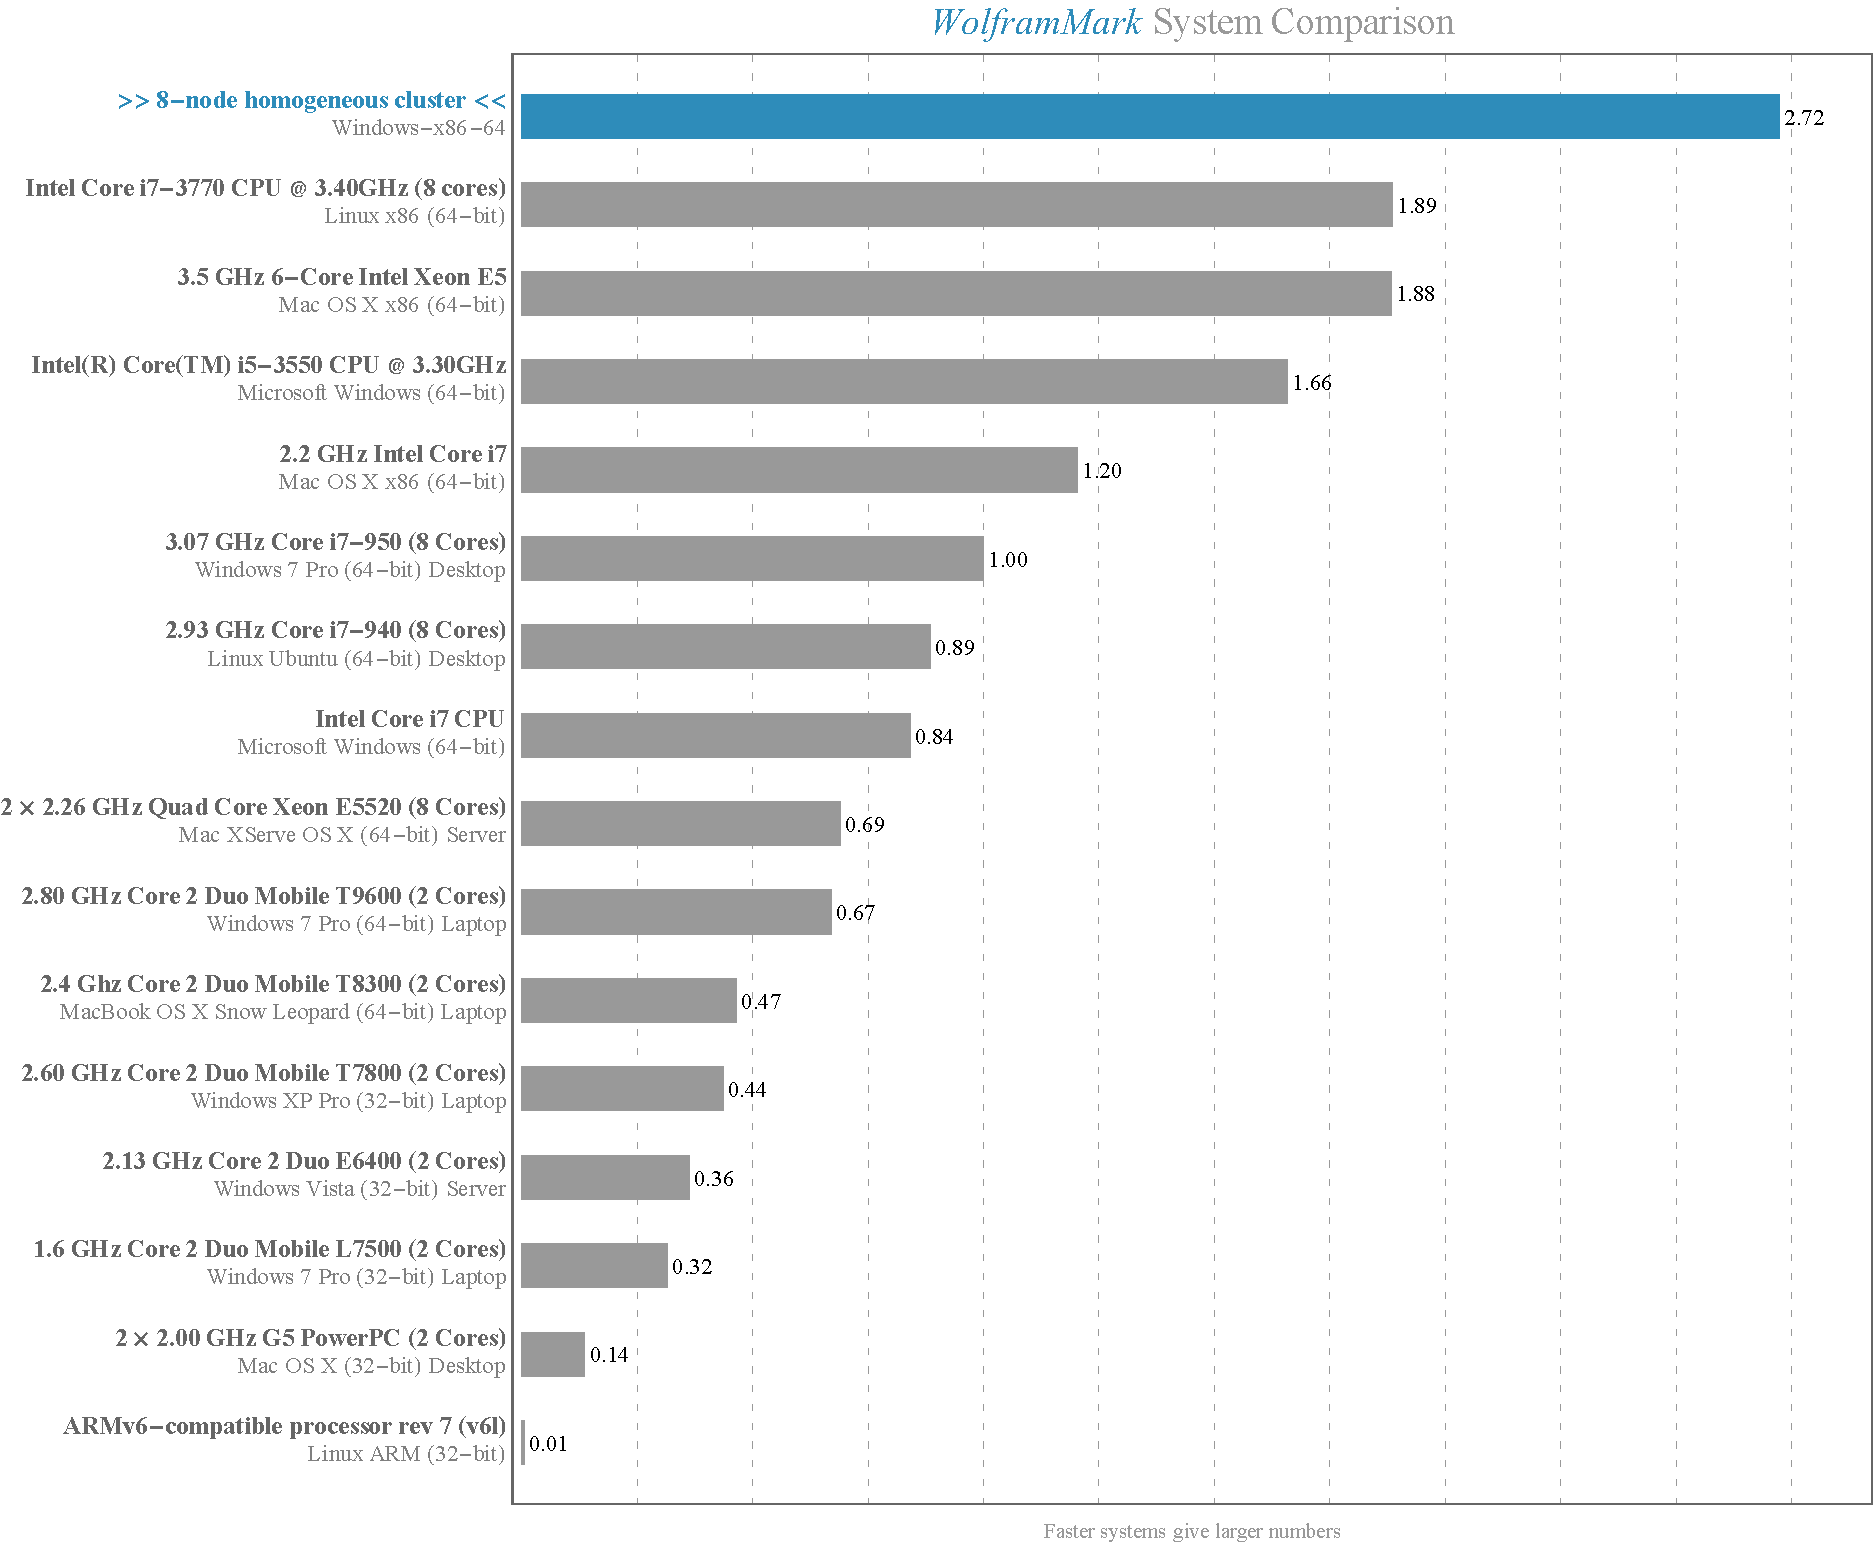
\includegraphics[width=\textwidth]{2}}
\caption{второй  попавшийся график}
\label{fig:2}
\end{figure}
\subsection{Ссылки}

В LaTeX можно создать ссылку почти на любой объект имеющий номер --- на раздел, рисунок, формулу, пункт списка и т. п. При этом LaTeX сам позаботится о нумерации ссылок и ее обновлении по мере необходимости.\\
Команд для работы со ссылками всего три: $\backslash$label, $\backslash$ref и $\backslash$pageref, и они не зависят от того, на какой объект вы ссылаетесь.

С помощью $\backslash$label\{имя\} вы даете имя объекту, на который хотите сослаться --- помечаете его. В качестве примера были созданы формулы равнее
Чтобы сослаться на отмеченный объект используется команда $\backslash$ref\{имя\}. На ее месте в тексте документа будет напечатан номер, присвоенный объекту LaTeX'ом. Так, поставив ссылку на указанную выше формулу мы увидим: \ref{2}, хотя в исходном тексте документа стояло: $\backslash$ref\{2\}.\\
Наконец, команда $\backslash$pageref\{имя\} печатает номер страницы, на которой расположен объект с данным именем.\\
LaTeX Warning: Label(s) may have changed. Rerun to get cross-references right.
С помощью команды \pageref вы можете указать читателю номер страницы, на которой находится интересующий его объект. Например, указав в файле .tex:
См. формулу~($\backslash$ref\{2\}) на с.~$\backslash$pageref\{2\}.
получим в готовом документе:\\
См. формулу~(\ref{2}) на с.~\pageref{2}.
Так же делаются ссылки на граф. объекты например на график ~\ref{fig:2} на с.~\pageref{fig:2}.

\chapter{Практика 3}
\subsection{Задание}
\begin{enumerate}
\item Ликвидация долгов с начала семестра (дальше значение баллов будет принимать отрицательные значения!) 
\item Создать статью со встроенной библиографией 
\item Создать документ с внешней библиографией 
\end{enumerate}
\subsection{О Выполнении}
Итак так как надо создать 2 документа с разными типами библиографий то в этом документе будет содержаться внешняя библиография, А в папке с проектом будет написанна "Статья" с теоретической частью по внутренней библиографии и  содержащая её же (библиографию).
\section{Теоретическая часть внешней библиографии (BibTeX)}
В подавляющем объеме случаев для создания внешней библиографии используется bibtex.\\
Далее текст взят из \cite{wiki1} и отредактирован.\\
BibTeX — программное обеспечение для создания форматированных списков библиографии. BibTeX используется совместно с LaTeX'ом и входит во все известные дистрибутивы TeX и LaTeX.
\subsection{Использование}
При подготовке документа в LaTeX система BibTeX предоставляет по сравнению со стандартным LaTeX-окружением thebibliography следующие преимущества:
\begin{itemize}
\item список литературы генерируется автоматически по всем ссылкам \cite, упомянутым в тексте;
\item можно использовать единую библиографическую базу (bib-файл) во всех своих текстах, во всех работах отдела, и т. д.;
\item легко обмениваться библиографическими базами с коллегами;
\item нет необходимости помнить правила оформления библиографии, так как BibTeX делает эту работу автоматически с помощью стилевых bst-файлов.
\end{itemize}
Для вызова BibTeX’а достаточно заменить окружение thebibliography командами\\

$\backslash$bibliographystyle{stylefile} \\
bst-файл, задающий стиль оформления библиографии\\

$\backslash$bibliography{bibfile} \\
имя bib-файла, содержащего библиографическую базу\\

Можно использовать несколько библиографических баз одновременно (тогда их имена указываются через запятую).\\

BibTeX использует bst-файлы для описания того, как bib-записи преобразуются в текст на LaTeX'e. Каждый bst-файл представляет собой программу на простом стековом языке программирования, напоминающем Forth или PostScript. Есть программы, позволяющие генерировать .bst-файлы автоматически (например, custom-bib или Bib-it).\\

Далее вставлен pdf файл представляющий из себя статью с внутренней библиографией\\
 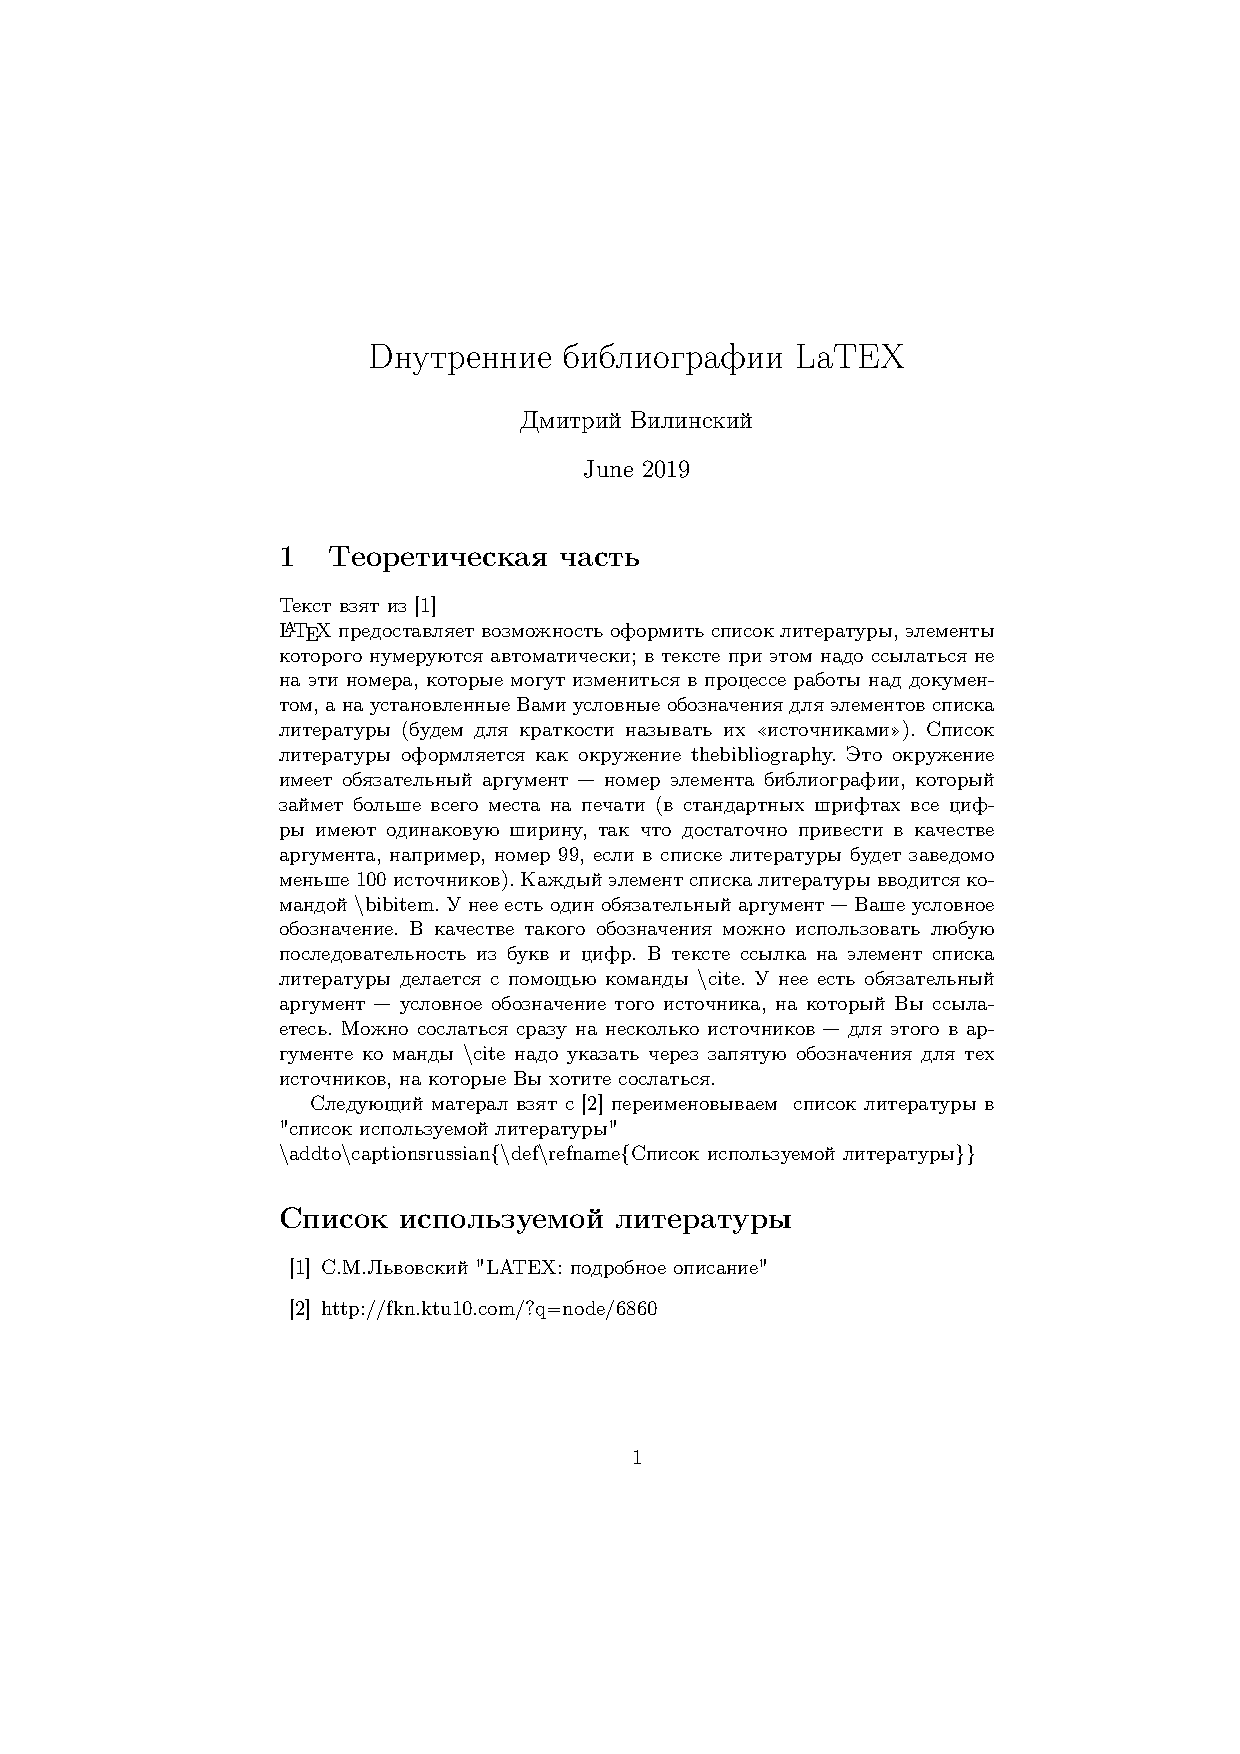
\includepdf[pages=-]{Bibl.pdf}



\chapter{Практика 4}
\subsection{Задание}
\begin{itemize}
\item По материалам статьи создать документ их шаблона Презентация 
\item Повторить все основные элементы статьи в презентации 
\end{itemize}
\section{О Выполнении}
Задание недоконца осознанно поэтому будет выполнеенно следующим образом:\\
В отдельном tex файле будет созданна презентация по теме создание презентаций на \LaTeX{} после чего скомпилирована в PDF и вставленна сюда.\\
Вот Она созданна с помошью \cite{pres1}
 
\includepdf[pages=-]{Pres.pdf}

\chapter{Практика 5}
\subsection{Задание}

\begin{itemize}
\item Для публикации использовать шаблон "Тезис" (Диссертация) 
\item Оформить титульный лист, разбивку на главы, внешний список литературы 
\end{itemize}

\section{О Выполнении}
С Шаблоном "Тезис" возникла проблема ибо в стандартных я такого ненашел, а это значит , что его надо или писать самому или искать готовый я пошел по второму пути
в результате шблон был добавлен в проект. Взят он был  с Сайта УрФу из раздела с описанием требований к ВКР, Конечно это не гарантирует соответсвие требованием Нормоконтроля, но ближе к ним вряд ли удастся подобраться.

\subsection{Оглавление}
В процессе работы LATEX автоматически собирает информацию для создания оглавления и
записывает ее в специальный файл с тем же именем, что у обрабатываемого файла, и расши
рением toc. Чтобы LATEX записал эту информацию, а затем воспользовался ею и напечатал
оглавление, надо дать команду $\backslash$tableofcontents.
Стало быть, оглавление, генерируемое LATEXом, всякий раз будет «на шаг отставать» от
реального положения дел. Чтобы учесть все возможные изменения и получить верное оглав
ление, надо будет в самом конце работы над текстом запустить LATEX еще раз (напоминания
об этом LATEX не выдаст).

\chapter{Практика 6}
\subsection{Залание}
\begin{enumerate}
\item Найти правила оформления выпускной работы магистра в этом году (или прошлом). Написать список различий готового шаблоны с требуемым 
\item  Написать предложения с описанием технологий исправлений (возможно найти готовые шаблоны, подходящие для целей)
\end{enumerate}
\section{выполнение}
Как было сказанно в прошлом пукте шаблон ВКФ был взят с Сайта УрФУ так что различий с требованиями никакх
Если понадобиться то в шаблоне давольно явно указанны параметры и их можно будет заменить

\chapter{Практика 7}
\subsection{Залание}
\begin{enumerate}
\item Описание на своей странице технологии написания пользовательских команд (макросов) в документе 
\item Придумать и реализовать 2-3 макроса в своей диссертации 
\end{enumerate}
\section{Макросы}
Для создания макросов используется команда $\backslash$newcommand. Эта команда имеет два обя
зательных аргумента. Первый из них — имя, которое Вы придумали для Вашего макроса.
Имена макросов должны подчиняться тем же правилам, что имена TEXовских команд : либо backslash и после него одна не-буква, либо backslash и после него — последовательность букв. Второй 37обязательный аргумент команды $\backslash$newcommand, называемый «замещающим текстом», сообщает TEXу смысл макроса: на этот текст Ваш макрос будет
замещаться в процессе трансляции (как говорят, макрос будет «разворачиваться»).

Приведем пару примеров он же будут выполнением 3-го пункта задания

$\backslash$newcommand\{$\backslash$ВКР\}\{\{Выпускная квалификационная работа\}\}\\

\newcommand{\ВКР}{{Выпускная квалификационная работа }}\\
Введя \\
Эта $\backslash$ВКР оформленна как надо\\
мы получим \\
Эта \ВКР   оформленна как надо\\
Макросы с переменными  \\
например введем макрос для символа Лежандра \[ \left(\frac{a}{b}\right) \]

$\backslash$newcommand\{\SIMWOL\}[2]\{$\backslash$left($\backslash$frac\{\#1\}\{\#2\}$\backslash$right)\}
\newcommand{\SIMWOL}[2]{\left(\frac{#1}{#2}\right)}\\
При записи $\backslash$SIMWOL\{a+b\}\{c+d\}
\[\SIMWOL{a+b}{c+d}
\]

\chapter{Практика 8}
\subsection{Залание}
\begin{enumerate}
\item Изменить титульный лист шаблона "Тезис" в соответствии с требованиями УрФУ 
\item Проверить названия разделов диссертации, продемонстрировать правильно оформленный список литературы 
\end{enumerate}
\section{выполнение}
Титульный лист опять же был взят из образца \cite{UrFU}
Название статей проверенны но со списком есть некоторые проблемы в плане отображения ссылок
\chapter{Практика 9}
\subsection{Залание}
\begin{enumerate}
\item Выполнить требования выпускной работы к шрифтам и полям страницы 
\item Выполнить требования выпускной работы к межстрочному интервалу 
\end{enumerate}
\section{выполнение}
Шрифты устанавливаются последовательностю команд. \\
$\backslash$usepackage\{fontspec\} 
\par \hfill {\ttfamily подготавливает загрузку шрифтов Open Type, True Type и др.}\\
$\backslash$defaultfontfeatures\{Ligatures=\{TeX\},Renderer=Basic\}
\par \hfill  {\ttfamily свойства шрифтов по умолчанию}\\
$\backslash$setmainfont[Ligatures=\{TeX,Historic\}]\{Times New Roman\} \par \hfill {\ttfamily задаёт основной шрифт документа}\\
$\backslash$setsansfont\{Comic Sans MS\}                  \par\hfill {\ttfamily задаёт шрифт без засечек}\\
$\backslash$setmonofont\{Courier New\}


$\backslash$ usepackage\{geometry\}  \hfill {\ttfamily Простой способ установления полей}\\
    $\backslash$ geometry\{top=25mm\}\\
    $\backslash$ geometry\{bottom=35mm\}\\
    $\backslash$ geometry\{left=35mm\}\\
    $\backslash$ geometry\{right=20mm\}\\

 $\backslash$ usepackage\{setspace\} \hfill {\ttfamily Интерлиньяж}\\  
 $\backslash$ onehalfspacing \hfill {\ttfamily Интерлиньяж 1.5}\\  



\bibliography{Bibl} 
\bibliographystyle{gost2008ls}





\end{document}









